\documentclass[1p]{elsarticle_modified}
%\bibliographystyle{elsarticle-num}

%\usepackage[colorlinks]{hyperref}
%\usepackage{abbrmath_seonhwa} %\Abb, \Ascr, \Acal ,\Abf, \Afrak
\usepackage{amsfonts}
\usepackage{amssymb}
\usepackage{amsmath}
\usepackage{amsthm}
\usepackage{scalefnt}
\usepackage{amsbsy}
\usepackage{kotex}
\usepackage{caption}
\usepackage{subfig}
\usepackage{color}
\usepackage{graphicx}
\usepackage{xcolor} %% white, black, red, green, blue, cyan, magenta, yellow
\usepackage{float}
\usepackage{setspace}
\usepackage{hyperref}

\usepackage{tikz}
\usetikzlibrary{arrows}

\usepackage{multirow}
\usepackage{array} % fixed length table
\usepackage{hhline}

%%%%%%%%%%%%%%%%%%%%%
\makeatletter
\renewcommand*\env@matrix[1][\arraystretch]{%
	\edef\arraystretch{#1}%
	\hskip -\arraycolsep
	\let\@ifnextchar\new@ifnextchar
	\array{*\c@MaxMatrixCols c}}
\makeatother %https://tex.stackexchange.com/questions/14071/how-can-i-increase-the-line-spacing-in-a-matrix
%%%%%%%%%%%%%%%

\usepackage[normalem]{ulem}

\newcommand{\msout}[1]{\ifmmode\text{\sout{\ensuremath{#1}}}\else\sout{#1}\fi}
%SOURCE: \msout is \stkout macro in https://tex.stackexchange.com/questions/20609/strikeout-in-math-mode

\newcommand{\cancel}[1]{
	\ifmmode
	{\color{red}\msout{#1}}
	\else
	{\color{red}\sout{#1}}
	\fi
}

\newcommand{\add}[1]{
	{\color{blue}\uwave{#1}}
}

\newcommand{\replace}[2]{
	\ifmmode
	{\color{red}\msout{#1}}{\color{blue}\uwave{#2}}
	\else
	{\color{red}\sout{#1}}{\color{blue}\uwave{#2}}
	\fi
}

\newcommand{\Sol}{\mathcal{S}} %segment
\newcommand{\D}{D} %diagram
\newcommand{\A}{\mathcal{A}} %arc


%%%%%%%%%%%%%%%%%%%%%%%%%%%%%5 test

\def\sl{\operatorname{\textup{SL}}(2,\Cbb)}
\def\psl{\operatorname{\textup{PSL}}(2,\Cbb)}
\def\quan{\mkern 1mu \triangleright \mkern 1mu}

\theoremstyle{definition}
\newtheorem{thm}{Theorem}[section]
\newtheorem{prop}[thm]{Proposition}
\newtheorem{lem}[thm]{Lemma}
\newtheorem{ques}[thm]{Question}
\newtheorem{cor}[thm]{Corollary}
\newtheorem{defn}[thm]{Definition}
\newtheorem{exam}[thm]{Example}
\newtheorem{rmk}[thm]{Remark}
\newtheorem{alg}[thm]{Algorithm}

\newcommand{\I}{\sqrt{-1}}
\begin{document}

%\begin{frontmatter}
%
%\title{Boundary parabolic representations of knots up to 8 crossings}
%
%%% Group authors per affiliation:
%\author{Yunhi Cho} 
%\address{Department of Mathematics, University of Seoul, Seoul, Korea}
%\ead{yhcho@uos.ac.kr}
%
%
%\author{Seonhwa Kim} %\fnref{s_kim}}
%\address{Center for Geometry and Physics, Institute for Basic Science, Pohang, 37673, Korea}
%\ead{ryeona17@ibs.re.kr}
%
%\author{Hyuk Kim}
%\address{Department of Mathematical Sciences, Seoul National University, Seoul 08826, Korea}
%\ead{hyukkim@snu.ac.kr}
%
%\author{Seokbeom Yoon}
%\address{Department of Mathematical Sciences, Seoul National University, Seoul, 08826,  Korea}
%\ead{sbyoon15@snu.ac.kr}
%
%\begin{abstract}
%We find all boundary parabolic representation of knots up to 8 crossings.
%
%\end{abstract}
%\begin{keyword}
%    \MSC[2010] 57M25 
%\end{keyword}
%
%\end{frontmatter}

%\linenumbers
%\tableofcontents
%
\newcommand\colored[1]{\textcolor{white}{\rule[-0.35ex]{0.8em}{1.4ex}}\kern-0.8em\color{red} #1}%
%\newcommand\colored[1]{\textcolor{white}{ #1}\kern-2.17ex	\textcolor{white}{ #1}\kern-1.81ex	\textcolor{white}{ #1}\kern-2.15ex\color{red}#1	}

{\Large $\underline{12a_{0412}~(K12a_{0412})}$}

\setlength{\tabcolsep}{10pt}
\renewcommand{\arraystretch}{1.6}
\vspace{1cm}\begin{tabular}{m{100pt}>{\centering\arraybackslash}m{274pt}}
\multirow{5}{120pt}{
	\centering
	\includegraphics[width=112pt]{../../../GIT/diagram.site/Diagrams/png/1213_12a_0412.png}\\
\ \ \ A knot diagram\footnotemark}&
\allowdisplaybreaks
\textbf{Linearized knot diagam} \\
\cline{2-2}
 &
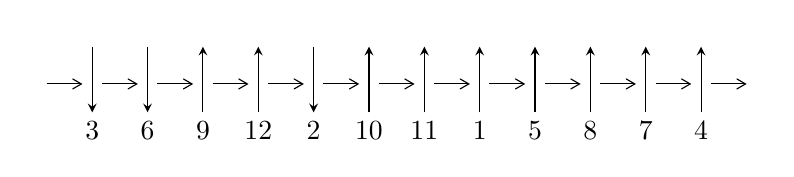
\begin{tikzpicture}[x=20pt, y=17pt]
	% nodes
	\node (C0) at (0, 0) {};
	\node (C1) at (1, 0) {};
	\node (C1U) at (1, +1) {};
	\node (C1D) at (1, -1) {3};

	\node (C2) at (2, 0) {};
	\node (C2U) at (2, +1) {};
	\node (C2D) at (2, -1) {6};

	\node (C3) at (3, 0) {};
	\node (C3U) at (3, +1) {};
	\node (C3D) at (3, -1) {9};

	\node (C4) at (4, 0) {};
	\node (C4U) at (4, +1) {};
	\node (C4D) at (4, -1) {12};

	\node (C5) at (5, 0) {};
	\node (C5U) at (5, +1) {};
	\node (C5D) at (5, -1) {2};

	\node (C6) at (6, 0) {};
	\node (C6U) at (6, +1) {};
	\node (C6D) at (6, -1) {10};

	\node (C7) at (7, 0) {};
	\node (C7U) at (7, +1) {};
	\node (C7D) at (7, -1) {11};

	\node (C8) at (8, 0) {};
	\node (C8U) at (8, +1) {};
	\node (C8D) at (8, -1) {1};

	\node (C9) at (9, 0) {};
	\node (C9U) at (9, +1) {};
	\node (C9D) at (9, -1) {5};

	\node (C10) at (10, 0) {};
	\node (C10U) at (10, +1) {};
	\node (C10D) at (10, -1) {8};

	\node (C11) at (11, 0) {};
	\node (C11U) at (11, +1) {};
	\node (C11D) at (11, -1) {7};

	\node (C12) at (12, 0) {};
	\node (C12U) at (12, +1) {};
	\node (C12D) at (12, -1) {4};
	\node (C13) at (13, 0) {};

	% arrows
	\draw[->,>={angle 60}]
	(C0) edge (C1) (C1) edge (C2) (C2) edge (C3) (C3) edge (C4) (C4) edge (C5) (C5) edge (C6) (C6) edge (C7) (C7) edge (C8) (C8) edge (C9) (C9) edge (C10) (C10) edge (C11) (C11) edge (C12) (C12) edge (C13) ;	\draw[->,>=stealth]
	(C1U) edge (C1D) (C2U) edge (C2D) (C3D) edge (C3U) (C4D) edge (C4U) (C5U) edge (C5D) (C6D) edge (C6U) (C7D) edge (C7U) (C8D) edge (C8U) (C9D) edge (C9U) (C10D) edge (C10U) (C11D) edge (C11U) (C12D) edge (C12U) ;
	\end{tikzpicture} \\
\hhline{~~} \\& 
\textbf{Solving Sequence} \\ \cline{2-2} 
 &
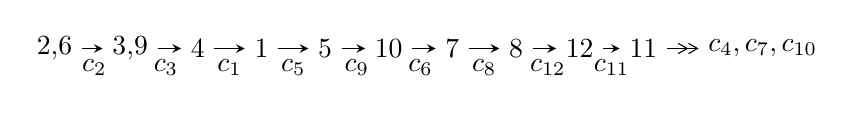
\begin{tikzpicture}[x=23pt, y=7pt]
	% node
	\node (A0) at (-1/8, 0) {2,6};
	\node (A1) at (17/16, 0) {3,9};
	\node (A2) at (17/8, 0) {4};
	\node (A3) at (25/8, 0) {1};
	\node (A4) at (33/8, 0) {5};
	\node (A5) at (41/8, 0) {10};
	\node (A6) at (49/8, 0) {7};
	\node (A7) at (57/8, 0) {8};
	\node (A8) at (65/8, 0) {12};
	\node (A9) at (73/8, 0) {11};
	\node (C1) at (1/2, -1) {$c_{2}$};
	\node (C2) at (13/8, -1) {$c_{3}$};
	\node (C3) at (21/8, -1) {$c_{1}$};
	\node (C4) at (29/8, -1) {$c_{5}$};
	\node (C5) at (37/8, -1) {$c_{9}$};
	\node (C6) at (45/8, -1) {$c_{6}$};
	\node (C7) at (53/8, -1) {$c_{8}$};
	\node (C8) at (61/8, -1) {$c_{12}$};
	\node (C9) at (69/8, -1) {$c_{11}$};
	\node (A10) at (11, 0) {$c_{4},c_{7},c_{10}$};

	% edge
	\draw[->,>=stealth]	
	(A0) edge (A1) (A1) edge (A2) (A2) edge (A3) (A3) edge (A4) (A4) edge (A5) (A5) edge (A6) (A6) edge (A7) (A7) edge (A8) (A8) edge (A9) ;
	\draw[->>,>={angle 60}]	
	(A9) edge (A10);
\end{tikzpicture} \\ 

\end{tabular} \\

\footnotetext{
The image of knot diagram is generated by the software ``\textbf{Draw programme}" developed by Andrew Bartholomew(\url{http://www.layer8.co.uk/maths/draw/index.htm\#Running-draw}), where we modified some parts for our purpose(\url{https://github.com/CATsTAILs/LinksPainter}).
}\phantom \\ \newline 
\centering \textbf{Ideals for irreducible components\footnotemark of $X_{\text{par}}$} 
 
\begin{align*}
I^u_{1}&=\langle 
4.20170\times10^{176} u^{104}-3.69872\times10^{177} u^{103}+\cdots+1.98967\times10^{177} b-1.56965\times10^{177},\\
\phantom{I^u_{1}}&\phantom{= \langle  }-1.93657\times10^{177} u^{104}+3.13804\times10^{178} u^{103}+\cdots+2.18864\times10^{178} a-3.72446\times10^{178},\\
\phantom{I^u_{1}}&\phantom{= \langle  }u^{105}-7 u^{104}+\cdots+3 u+1\rangle \\
\\
\end{align*}
\raggedright * 1 irreducible components of $\dim_{\mathbb{C}}=0$, with total 105 representations.\\
\footnotetext{All coefficients of polynomials are rational numbers. But the coefficients are sometimes approximated in decimal forms when there is not enough margin.}
\newpage
\renewcommand{\arraystretch}{1}
\centering \section*{I. $I^u_{1}= \langle 4.20\times10^{176} u^{104}-3.70\times10^{177} u^{103}+\cdots+1.99\times10^{177} b-1.57\times10^{177},\;-1.94\times10^{177} u^{104}+3.14\times10^{178} u^{103}+\cdots+2.19\times10^{178} a-3.72\times10^{178},\;u^{105}-7 u^{104}+\cdots+3 u+1 \rangle$}
\flushleft \textbf{(i) Arc colorings}\\
\begin{tabular}{m{7pt} m{180pt} m{7pt} m{180pt} }
\flushright $a_{2}=$&$\begin{pmatrix}1\\0\end{pmatrix}$ \\
\flushright $a_{6}=$&$\begin{pmatrix}0\\u\end{pmatrix}$ \\
\flushright $a_{3}=$&$\begin{pmatrix}1\\u^2\end{pmatrix}$ \\
\flushright $a_{9}=$&$\begin{pmatrix}0.0884829 u^{104}-1.43379 u^{103}+\cdots+0.687210 u+1.70173\\-0.211175 u^{104}+1.85896 u^{103}+\cdots+0.342478 u+0.788902\end{pmatrix}$ \\
\flushright $a_{4}=$&$\begin{pmatrix}-0.165696 u^{104}-0.198162 u^{103}+\cdots-5.72062 u-1.82003\\0.0402541 u^{104}-0.944412 u^{103}+\cdots-2.78766 u-0.617942\end{pmatrix}$ \\
\flushright $a_{1}=$&$\begin{pmatrix}- u^2+1\\- u^4\end{pmatrix}$ \\
\flushright $a_{5}=$&$\begin{pmatrix}u\\u\end{pmatrix}$ \\
\flushright $a_{10}=$&$\begin{pmatrix}2.15833 u^{104}-14.1242 u^{103}+\cdots-2.59855 u+0.506586\\1.85867 u^{104}-10.8314 u^{103}+\cdots-2.94328 u-0.406239\end{pmatrix}$ \\
\flushright $a_{7}=$&$\begin{pmatrix}1.13726 u^{104}-6.38343 u^{103}+\cdots-8.00594 u-2.72657\\0.380524 u^{104}-2.29143 u^{103}+\cdots+3.83633 u+0.123900\end{pmatrix}$ \\
\flushright $a_{8}=$&$\begin{pmatrix}2.25309 u^{104}-14.9010 u^{103}+\cdots-2.19648 u-0.0146111\\1.96367 u^{104}-11.9280 u^{103}+\cdots-5.85996 u-0.890655\end{pmatrix}$ \\
\flushright $a_{12}=$&$\begin{pmatrix}1.97598 u^{104}-11.9594 u^{103}+\cdots-9.62283 u-1.09953\\2.39398 u^{104}-15.0162 u^{103}+\cdots-6.27032 u-2.03812\end{pmatrix}$ \\
\flushright $a_{11}=$&$\begin{pmatrix}1.58757 u^{104}-9.31152 u^{103}+\cdots+0.980426 u+1.41068\\1.26723 u^{104}-7.07029 u^{103}+\cdots-0.922253 u-0.284019\end{pmatrix}$\\&\end{tabular}
\flushleft \textbf{(ii) Obstruction class $= -1$}\\~\\
\flushleft \textbf{(iii) Cusp Shapes $= 5.01196 u^{104}-31.9283 u^{103}+\cdots-6.46734 u+9.94137$}\\~\\
\newpage\renewcommand{\arraystretch}{1}
\flushleft \textbf{(iv) u-Polynomials at the component}\newline \\
\begin{tabular}{m{50pt}|m{274pt}}
Crossings & \hspace{64pt}u-Polynomials at each crossing \\
\hline $$\begin{aligned}c_{1}\end{aligned}$$&$\begin{aligned}
&u^{105}+41 u^{104}+\cdots+13 u+1
\end{aligned}$\\
\hline $$\begin{aligned}c_{2},c_{5}\end{aligned}$$&$\begin{aligned}
&u^{105}+7 u^{104}+\cdots+3 u-1
\end{aligned}$\\
\hline $$\begin{aligned}c_{3}\end{aligned}$$&$\begin{aligned}
&u^{105}- u^{104}+\cdots-3 u-1
\end{aligned}$\\
\hline $$\begin{aligned}c_{4},c_{12}\end{aligned}$$&$\begin{aligned}
&u^{105}+7 u^{104}+\cdots+3 u-1
\end{aligned}$\\
\hline $$\begin{aligned}c_{6}\end{aligned}$$&$\begin{aligned}
&u^{105}- u^{104}+\cdots+625275 u-85457
\end{aligned}$\\
\hline $$\begin{aligned}c_{7},c_{10},c_{11}\end{aligned}$$&$\begin{aligned}
&u^{105}+u^{104}+\cdots+u-1
\end{aligned}$\\
\hline $$\begin{aligned}c_{8}\end{aligned}$$&$\begin{aligned}
&u^{105}+3 u^{104}+\cdots-31 u-3
\end{aligned}$\\
\hline $$\begin{aligned}c_{9}\end{aligned}$$&$\begin{aligned}
&u^{105}+u^{104}+\cdots+413 u-2359
\end{aligned}$\\
\hline
\end{tabular}\\~\\
\newpage\renewcommand{\arraystretch}{1}
\flushleft \textbf{(v) Riley Polynomials at the component}\newline \\
\begin{tabular}{m{50pt}|m{274pt}}
Crossings & \hspace{64pt}Riley Polynomials at each crossing \\
\hline $$\begin{aligned}c_{1}\end{aligned}$$&$\begin{aligned}
&y^{105}+47 y^{104}+\cdots+245 y-1
\end{aligned}$\\
\hline $$\begin{aligned}c_{2},c_{5}\end{aligned}$$&$\begin{aligned}
&y^{105}-41 y^{104}+\cdots+13 y-1
\end{aligned}$\\
\hline $$\begin{aligned}c_{3}\end{aligned}$$&$\begin{aligned}
&y^{105}+7 y^{104}+\cdots+69 y-1
\end{aligned}$\\
\hline $$\begin{aligned}c_{4},c_{12}\end{aligned}$$&$\begin{aligned}
&y^{105}+67 y^{104}+\cdots+13 y-1
\end{aligned}$\\
\hline $$\begin{aligned}c_{6}\end{aligned}$$&$\begin{aligned}
&y^{105}-25 y^{104}+\cdots+228484645933 y-7302898849
\end{aligned}$\\
\hline $$\begin{aligned}c_{7},c_{10},c_{11}\end{aligned}$$&$\begin{aligned}
&y^{105}+91 y^{104}+\cdots+45 y-1
\end{aligned}$\\
\hline $$\begin{aligned}c_{8}\end{aligned}$$&$\begin{aligned}
&y^{105}+231 y^{104}+\cdots-3743 y-9
\end{aligned}$\\
\hline $$\begin{aligned}c_{9}\end{aligned}$$&$\begin{aligned}
&y^{105}-209 y^{104}+\cdots+318380797 y-5564881
\end{aligned}$\\
\hline
\end{tabular}\\~\\
\newpage\flushleft \textbf{(vi) Complex Volumes and Cusp Shapes}
$$\begin{array}{c|c|c}  
\text{Solutions to }I^u_{1}& \I (\text{vol} + \sqrt{-1}CS) & \text{Cusp shape}\\
 \hline 
\begin{aligned}
u &= -0.784644 + 0.598937 I \\
a &= \phantom{-}2.25636 - 0.88903 I \\
b &= \phantom{-}1.36159 - 1.31807 I\end{aligned}
 & \phantom{-}1.85369 - 0.14305 I & \phantom{-0.000000 } 0 \\ \hline\begin{aligned}
u &= -0.784644 - 0.598937 I \\
a &= \phantom{-}2.25636 + 0.88903 I \\
b &= \phantom{-}1.36159 + 1.31807 I\end{aligned}
 & \phantom{-}1.85369 + 0.14305 I & \phantom{-0.000000 } 0 \\ \hline\begin{aligned}
u &= -0.858240 + 0.539535 I \\
a &= \phantom{-}7.28815 + 2.86509 I \\
b &= \phantom{-}6.10302 - 5.61999 I\end{aligned}
 & -4.68800 - 0.72454 I & \phantom{-0.000000 } 0 \\ \hline\begin{aligned}
u &= -0.858240 - 0.539535 I \\
a &= \phantom{-}7.28815 - 2.86509 I \\
b &= \phantom{-}6.10302 + 5.61999 I\end{aligned}
 & -4.68800 + 0.72454 I & \phantom{-0.000000 } 0 \\ \hline\begin{aligned}
u &= \phantom{-}0.564992 + 0.806358 I \\
a &= -0.88945 - 1.11350 I \\
b &= \phantom{-}0.24954 - 1.51542 I\end{aligned}
 & -0.43187 + 4.02094 I & \phantom{-0.000000 } 0 \\ \hline\begin{aligned}
u &= \phantom{-}0.564992 - 0.806358 I \\
a &= -0.88945 + 1.11350 I \\
b &= \phantom{-}0.24954 + 1.51542 I\end{aligned}
 & -0.43187 - 4.02094 I & \phantom{-0.000000 } 0 \\ \hline\begin{aligned}
u &= -0.881792 + 0.510724 I \\
a &= -10.51730 + 2.00682 I \\
b &= -3.80678 + 10.52150 I\end{aligned}
 & -0.56771 + 2.03241 I & \phantom{-0.000000 } 0 \\ \hline\begin{aligned}
u &= -0.881792 - 0.510724 I \\
a &= -10.51730 - 2.00682 I \\
b &= -3.80678 - 10.52150 I\end{aligned}
 & -0.56771 - 2.03241 I & \phantom{-0.000000 } 0 \\ \hline\begin{aligned}
u &= \phantom{-}0.387986 + 0.950406 I \\
a &= \phantom{-}0.482022 - 0.428068 I \\
b &= \phantom{-}0.468486 + 0.163848 I\end{aligned}
 & \phantom{-}0.84097 - 3.95845 I & \phantom{-0.000000 } 0 \\ \hline\begin{aligned}
u &= \phantom{-}0.387986 - 0.950406 I \\
a &= \phantom{-}0.482022 + 0.428068 I \\
b &= \phantom{-}0.468486 - 0.163848 I\end{aligned}
 & \phantom{-}0.84097 + 3.95845 I & \phantom{-0.000000 } 0\\
 \hline 
 \end{array}$$\newpage$$\begin{array}{c|c|c}  
\text{Solutions to }I^u_{1}& \I (\text{vol} + \sqrt{-1}CS) & \text{Cusp shape}\\
 \hline 
\begin{aligned}
u &= -0.913124 + 0.476644 I \\
a &= \phantom{-}4.58490 - 3.63846 I \\
b &= -0.09300 - 6.06609 I\end{aligned}
 & -4.71244 + 4.76569 I & \phantom{-0.000000 } 0 \\ \hline\begin{aligned}
u &= -0.913124 - 0.476644 I \\
a &= \phantom{-}4.58490 + 3.63846 I \\
b &= -0.09300 + 6.06609 I\end{aligned}
 & -4.71244 - 4.76569 I & \phantom{-0.000000 } 0 \\ \hline\begin{aligned}
u &= \phantom{-}0.839840 + 0.597226 I \\
a &= -1.246410 + 0.445955 I \\
b &= -0.759419 + 0.644703 I\end{aligned}
 & \phantom{-}2.38346 - 2.36277 I & \phantom{-0.000000 } 0 \\ \hline\begin{aligned}
u &= \phantom{-}0.839840 - 0.597226 I \\
a &= -1.246410 - 0.445955 I \\
b &= -0.759419 - 0.644703 I\end{aligned}
 & \phantom{-}2.38346 + 2.36277 I & \phantom{-0.000000 } 0 \\ \hline\begin{aligned}
u &= \phantom{-}0.850571 + 0.587804 I \\
a &= -0.605447 + 0.275364 I \\
b &= -0.121760 + 0.829135 I\end{aligned}
 & \phantom{-}2.36909 - 2.33534 I & \phantom{-0.000000 } 0 \\ \hline\begin{aligned}
u &= \phantom{-}0.850571 - 0.587804 I \\
a &= -0.605447 - 0.275364 I \\
b &= -0.121760 - 0.829135 I\end{aligned}
 & \phantom{-}2.36909 + 2.33534 I & \phantom{-0.000000 } 0 \\ \hline\begin{aligned}
u &= \phantom{-}0.542109 + 0.888877 I \\
a &= \phantom{-}0.989633 + 0.984793 I \\
b &= -0.40355 + 1.51977 I\end{aligned}
 & \phantom{-}1.65020 + 8.48448 I & \phantom{-0.000000 } 0 \\ \hline\begin{aligned}
u &= \phantom{-}0.542109 - 0.888877 I \\
a &= \phantom{-}0.989633 - 0.984793 I \\
b &= -0.40355 - 1.51977 I\end{aligned}
 & \phantom{-}1.65020 - 8.48448 I & \phantom{-0.000000 } 0 \\ \hline\begin{aligned}
u &= \phantom{-}0.987126 + 0.357010 I \\
a &= \phantom{-}0.172002 - 0.826380 I \\
b &= \phantom{-}1.364530 - 0.094449 I\end{aligned}
 & -5.21470 - 0.78396 I & \phantom{-0.000000 } 0 \\ \hline\begin{aligned}
u &= \phantom{-}0.987126 - 0.357010 I \\
a &= \phantom{-}0.172002 + 0.826380 I \\
b &= \phantom{-}1.364530 + 0.094449 I\end{aligned}
 & -5.21470 + 0.78396 I & \phantom{-0.000000 } 0\\
 \hline 
 \end{array}$$\newpage$$\begin{array}{c|c|c}  
\text{Solutions to }I^u_{1}& \I (\text{vol} + \sqrt{-1}CS) & \text{Cusp shape}\\
 \hline 
\begin{aligned}
u &= \phantom{-}0.715044 + 0.618340 I \\
a &= -0.20679 - 1.46973 I \\
b &= \phantom{-}0.09366 - 1.70389 I\end{aligned}
 & -0.37710 + 2.65093 I & \phantom{-0.000000 } 0 \\ \hline\begin{aligned}
u &= \phantom{-}0.715044 - 0.618340 I \\
a &= -0.20679 + 1.46973 I \\
b &= \phantom{-}0.09366 + 1.70389 I\end{aligned}
 & -0.37710 - 2.65093 I & \phantom{-0.000000 } 0 \\ \hline\begin{aligned}
u &= \phantom{-}0.513664 + 0.931812 I \\
a &= -1.057000 - 0.935885 I \\
b &= \phantom{-}0.50411 - 1.49044 I\end{aligned}
 & -3.58129 + 12.58550 I & \phantom{-0.000000 } 0 \\ \hline\begin{aligned}
u &= \phantom{-}0.513664 - 0.931812 I \\
a &= -1.057000 + 0.935885 I \\
b &= \phantom{-}0.50411 + 1.49044 I\end{aligned}
 & -3.58129 - 12.58550 I & \phantom{-0.000000 } 0 \\ \hline\begin{aligned}
u &= -0.648758 + 0.845940 I \\
a &= \phantom{-}0.890042 - 0.645854 I \\
b &= \phantom{-}0.009504 - 1.305990 I\end{aligned}
 & \phantom{-}2.52519 + 1.13520 I & \phantom{-0.000000 } 0 \\ \hline\begin{aligned}
u &= -0.648758 - 0.845940 I \\
a &= \phantom{-}0.890042 + 0.645854 I \\
b &= \phantom{-}0.009504 + 1.305990 I\end{aligned}
 & \phantom{-}2.52519 - 1.13520 I & \phantom{-0.000000 } 0 \\ \hline\begin{aligned}
u &= -0.733179 + 0.561323 I \\
a &= \phantom{-}1.41999 - 0.77213 I \\
b &= \phantom{-}0.74850 - 1.44176 I\end{aligned}
 & \phantom{-}1.39941 + 0.38540 I & \phantom{-0.000000 } 0 \\ \hline\begin{aligned}
u &= -0.733179 - 0.561323 I \\
a &= \phantom{-}1.41999 + 0.77213 I \\
b &= \phantom{-}0.74850 + 1.44176 I\end{aligned}
 & \phantom{-}1.39941 - 0.38540 I & \phantom{-0.000000 } 0 \\ \hline\begin{aligned}
u &= -0.552779 + 0.925006 I \\
a &= -0.823336 + 0.551394 I \\
b &= \phantom{-}0.127984 + 1.085750 I\end{aligned}
 & \phantom{-}5.43319 - 2.63646 I & \phantom{-0.000000 } 0 \\ \hline\begin{aligned}
u &= -0.552779 - 0.925006 I \\
a &= -0.823336 - 0.551394 I \\
b &= \phantom{-}0.127984 - 1.085750 I\end{aligned}
 & \phantom{-}5.43319 + 2.63646 I & \phantom{-0.000000 } 0\\
 \hline 
 \end{array}$$\newpage$$\begin{array}{c|c|c}  
\text{Solutions to }I^u_{1}& \I (\text{vol} + \sqrt{-1}CS) & \text{Cusp shape}\\
 \hline 
\begin{aligned}
u &= -0.891298 + 0.610073 I \\
a &= -0.99689 + 1.67821 I \\
b &= -0.53902 + 2.37842 I\end{aligned}
 & \phantom{-}1.52100 + 4.93000 I & \phantom{-0.000000 } 0 \\ \hline\begin{aligned}
u &= -0.891298 - 0.610073 I \\
a &= -0.99689 - 1.67821 I \\
b &= -0.53902 - 2.37842 I\end{aligned}
 & \phantom{-}1.52100 - 4.93000 I & \phantom{-0.000000 } 0 \\ \hline\begin{aligned}
u &= \phantom{-}0.719718 + 0.566081 I \\
a &= \phantom{-}0.971659 + 0.472938 I \\
b &= -0.066367 - 0.169388 I\end{aligned}
 & -1.45824 + 1.82741 I & \phantom{-0.000000 } 0 \\ \hline\begin{aligned}
u &= \phantom{-}0.719718 - 0.566081 I \\
a &= \phantom{-}0.971659 - 0.472938 I \\
b &= -0.066367 + 0.169388 I\end{aligned}
 & -1.45824 - 1.82741 I & \phantom{-0.000000 } 0 \\ \hline\begin{aligned}
u &= -0.489338 + 0.987991 I \\
a &= \phantom{-}0.773874 - 0.512163 I \\
b &= -0.225468 - 0.939865 I\end{aligned}
 & \phantom{-}0.79628 - 6.39354 I & \phantom{-0.000000 } 0 \\ \hline\begin{aligned}
u &= -0.489338 - 0.987991 I \\
a &= \phantom{-}0.773874 + 0.512163 I \\
b &= -0.225468 + 0.939865 I\end{aligned}
 & \phantom{-}0.79628 + 6.39354 I & \phantom{-0.000000 } 0 \\ \hline\begin{aligned}
u &= \phantom{-}0.939075 + 0.580606 I \\
a &= \phantom{-}0.0878441 - 0.0304630 I \\
b &= -0.480576 - 0.945992 I\end{aligned}
 & -2.14023 - 6.43595 I & \phantom{-0.000000 } 0 \\ \hline\begin{aligned}
u &= \phantom{-}0.939075 - 0.580606 I \\
a &= \phantom{-}0.0878441 + 0.0304630 I \\
b &= -0.480576 + 0.945992 I\end{aligned}
 & -2.14023 + 6.43595 I & \phantom{-0.000000 } 0 \\ \hline\begin{aligned}
u &= -1.105020 + 0.003986 I \\
a &= -0.463514 + 0.579517 I \\
b &= -0.081000 - 0.445193 I\end{aligned}
 & -6.23158 - 2.80589 I & \phantom{-0.000000 } 0 \\ \hline\begin{aligned}
u &= -1.105020 - 0.003986 I \\
a &= -0.463514 - 0.579517 I \\
b &= -0.081000 + 0.445193 I\end{aligned}
 & -6.23158 + 2.80589 I & \phantom{-0.000000 } 0\\
 \hline 
 \end{array}$$\newpage$$\begin{array}{c|c|c}  
\text{Solutions to }I^u_{1}& \I (\text{vol} + \sqrt{-1}CS) & \text{Cusp shape}\\
 \hline 
\begin{aligned}
u &= -0.930889 + 0.606222 I \\
a &= -1.55877 + 0.85888 I \\
b &= -0.88224 + 1.58561 I\end{aligned}
 & \phantom{-}0.76571 + 4.31173 I & \phantom{-0.000000 } 0 \\ \hline\begin{aligned}
u &= -0.930889 - 0.606222 I \\
a &= -1.55877 - 0.85888 I \\
b &= -0.88224 - 1.58561 I\end{aligned}
 & \phantom{-}0.76571 - 4.31173 I & \phantom{-0.000000 } 0 \\ \hline\begin{aligned}
u &= \phantom{-}0.928998 + 0.618976 I \\
a &= \phantom{-}2.04545 + 0.23803 I \\
b &= \phantom{-}1.58004 + 0.66760 I\end{aligned}
 & -1.01275 - 7.53557 I & \phantom{-0.000000 } 0 \\ \hline\begin{aligned}
u &= \phantom{-}0.928998 - 0.618976 I \\
a &= \phantom{-}2.04545 - 0.23803 I \\
b &= \phantom{-}1.58004 - 0.66760 I\end{aligned}
 & -1.01275 + 7.53557 I & \phantom{-0.000000 } 0 \\ \hline\begin{aligned}
u &= \phantom{-}0.108711 + 0.871393 I \\
a &= -0.513219 + 0.308942 I \\
b &= -0.280446 + 0.170757 I\end{aligned}
 & -2.21809 - 1.17141 I & \phantom{-0.000000 } 0 \\ \hline\begin{aligned}
u &= \phantom{-}0.108711 - 0.871393 I \\
a &= -0.513219 - 0.308942 I \\
b &= -0.280446 - 0.170757 I\end{aligned}
 & -2.21809 + 1.17141 I & \phantom{-0.000000 } 0 \\ \hline\begin{aligned}
u &= \phantom{-}0.748138 + 0.456711 I \\
a &= -0.454893 + 1.287700 I \\
b &= -1.47842 + 0.24559 I\end{aligned}
 & -1.42263 - 2.10421 I & \phantom{-0.000000 } 0 \\ \hline\begin{aligned}
u &= \phantom{-}0.748138 - 0.456711 I \\
a &= -0.454893 - 1.287700 I \\
b &= -1.47842 - 0.24559 I\end{aligned}
 & -1.42263 + 2.10421 I & \phantom{-0.000000 } 0 \\ \hline\begin{aligned}
u &= \phantom{-}1.113190 + 0.197962 I \\
a &= \phantom{-}0.203752 + 0.323619 I \\
b &= \phantom{-}0.092885 - 0.183534 I\end{aligned}
 & -2.01882 - 1.15814 I & \phantom{-0.000000 } 0 \\ \hline\begin{aligned}
u &= \phantom{-}1.113190 - 0.197962 I \\
a &= \phantom{-}0.203752 - 0.323619 I \\
b &= \phantom{-}0.092885 + 0.183534 I\end{aligned}
 & -2.01882 + 1.15814 I & \phantom{-0.000000 } 0\\
 \hline 
 \end{array}$$\newpage$$\begin{array}{c|c|c}  
\text{Solutions to }I^u_{1}& \I (\text{vol} + \sqrt{-1}CS) & \text{Cusp shape}\\
 \hline 
\begin{aligned}
u &= -0.804192 + 0.313985 I \\
a &= -2.00216 + 0.54358 I \\
b &= -1.58425 + 1.27138 I\end{aligned}
 & -3.99118 - 2.00596 I & \phantom{-0.000000 } 0 \\ \hline\begin{aligned}
u &= -0.804192 - 0.313985 I \\
a &= -2.00216 - 0.54358 I \\
b &= -1.58425 - 1.27138 I\end{aligned}
 & -3.99118 + 2.00596 I & \phantom{-0.000000 } 0 \\ \hline\begin{aligned}
u &= \phantom{-}0.855335 + 0.112245 I \\
a &= \phantom{-}0.80652 + 1.60498 I \\
b &= \phantom{-}1.62206 + 1.22184 I\end{aligned}
 & -7.40410 + 4.25720 I & \phantom{-0.000000 } 0 \\ \hline\begin{aligned}
u &= \phantom{-}0.855335 - 0.112245 I \\
a &= \phantom{-}0.80652 - 1.60498 I \\
b &= \phantom{-}1.62206 - 1.22184 I\end{aligned}
 & -7.40410 - 4.25720 I & \phantom{-0.000000 } 0 \\ \hline\begin{aligned}
u &= -0.974317 + 0.592288 I \\
a &= \phantom{-}0.27144 - 1.61288 I \\
b &= \phantom{-}0.01068 - 2.47838 I\end{aligned}
 & -4.69892 + 9.33676 I & \phantom{-0.000000 } 0 \\ \hline\begin{aligned}
u &= -0.974317 - 0.592288 I \\
a &= \phantom{-}0.27144 + 1.61288 I \\
b &= \phantom{-}0.01068 + 2.47838 I\end{aligned}
 & -4.69892 - 9.33676 I & \phantom{-0.000000 } 0 \\ \hline\begin{aligned}
u &= -0.635040 + 0.567354 I \\
a &= -2.48560 + 0.33455 I \\
b &= -1.101240 + 0.509213 I\end{aligned}
 & -3.69404 - 4.64409 I & \phantom{-0.000000 } 0 \\ \hline\begin{aligned}
u &= -0.635040 - 0.567354 I \\
a &= -2.48560 - 0.33455 I \\
b &= -1.101240 - 0.509213 I\end{aligned}
 & -3.69404 + 4.64409 I & \phantom{-0.000000 } 0 \\ \hline\begin{aligned}
u &= \phantom{-}0.476371 + 1.053510 I \\
a &= -0.507456 + 0.437799 I \\
b &= -0.474779 - 0.347760 I\end{aligned}
 & -3.81811 - 7.20822 I & \phantom{-0.000000 } 0 \\ \hline\begin{aligned}
u &= \phantom{-}0.476371 - 1.053510 I \\
a &= -0.507456 - 0.437799 I \\
b &= -0.474779 + 0.347760 I\end{aligned}
 & -3.81811 + 7.20822 I & \phantom{-0.000000 } 0\\
 \hline 
 \end{array}$$\newpage$$\begin{array}{c|c|c}  
\text{Solutions to }I^u_{1}& \I (\text{vol} + \sqrt{-1}CS) & \text{Cusp shape}\\
 \hline 
\begin{aligned}
u &= -1.155890 + 0.151746 I \\
a &= \phantom{-}0.508318 - 0.111207 I \\
b &= \phantom{-}0.032423 + 0.975592 I\end{aligned}
 & -13.01170 - 1.06028 I & \phantom{-0.000000 } 0 \\ \hline\begin{aligned}
u &= -1.155890 - 0.151746 I \\
a &= \phantom{-}0.508318 + 0.111207 I \\
b &= \phantom{-}0.032423 - 0.975592 I\end{aligned}
 & -13.01170 + 1.06028 I & \phantom{-0.000000 } 0 \\ \hline\begin{aligned}
u &= -1.079920 + 0.483105 I \\
a &= \phantom{-}1.05608 - 1.02881 I \\
b &= \phantom{-}0.67251 - 1.36232 I\end{aligned}
 & -5.45759 + 5.13104 I & \phantom{-0.000000 } 0 \\ \hline\begin{aligned}
u &= -1.079920 - 0.483105 I \\
a &= \phantom{-}1.05608 + 1.02881 I \\
b &= \phantom{-}0.67251 + 1.36232 I\end{aligned}
 & -5.45759 - 5.13104 I & \phantom{-0.000000 } 0 \\ \hline\begin{aligned}
u &= \phantom{-}1.099770 + 0.484541 I \\
a &= \phantom{-}0.561303 + 0.185309 I \\
b &= \phantom{-}0.372907 + 0.221075 I\end{aligned}
 & -2.01746 - 1.41013 I & \phantom{-0.000000 } 0 \\ \hline\begin{aligned}
u &= \phantom{-}1.099770 - 0.484541 I \\
a &= \phantom{-}0.561303 - 0.185309 I \\
b &= \phantom{-}0.372907 - 0.221075 I\end{aligned}
 & -2.01746 + 1.41013 I & \phantom{-0.000000 } 0 \\ \hline\begin{aligned}
u &= -1.209830 + 0.064571 I \\
a &= \phantom{-}0.106577 + 0.547653 I \\
b &= -0.339099 - 0.297583 I\end{aligned}
 & -5.02520 + 6.71923 I & \phantom{-0.000000 } 0 \\ \hline\begin{aligned}
u &= -1.209830 - 0.064571 I \\
a &= \phantom{-}0.106577 - 0.547653 I \\
b &= -0.339099 + 0.297583 I\end{aligned}
 & -5.02520 - 6.71923 I & \phantom{-0.000000 } 0 \\ \hline\begin{aligned}
u &= \phantom{-}1.070970 + 0.573366 I \\
a &= -1.93630 - 0.77675 I \\
b &= -1.95721 - 1.69398 I\end{aligned}
 & -10.33900 - 8.37585 I & \phantom{-0.000000 } 0 \\ \hline\begin{aligned}
u &= \phantom{-}1.070970 - 0.573366 I \\
a &= -1.93630 + 0.77675 I \\
b &= -1.95721 + 1.69398 I\end{aligned}
 & -10.33900 + 8.37585 I & \phantom{-0.000000 } 0\\
 \hline 
 \end{array}$$\newpage$$\begin{array}{c|c|c}  
\text{Solutions to }I^u_{1}& \I (\text{vol} + \sqrt{-1}CS) & \text{Cusp shape}\\
 \hline 
\begin{aligned}
u &= \phantom{-}0.331960 + 0.691775 I \\
a &= \phantom{-}1.36501 + 1.42750 I \\
b &= -0.088717 + 1.079180 I\end{aligned}
 & -8.31773 + 3.57839 I & \phantom{-}0.49395 - 2.97375 I \\ \hline\begin{aligned}
u &= \phantom{-}0.331960 - 0.691775 I \\
a &= \phantom{-}1.36501 - 1.42750 I \\
b &= -0.088717 - 1.079180 I\end{aligned}
 & -8.31773 - 3.57839 I & \phantom{-}0.49395 + 2.97375 I \\ \hline\begin{aligned}
u &= -1.028750 + 0.688724 I \\
a &= -1.39282 + 0.64457 I \\
b &= -0.88861 + 1.57623 I\end{aligned}
 & \phantom{-}1.34242 + 4.57879 I & \phantom{-0.000000 } 0 \\ \hline\begin{aligned}
u &= -1.028750 - 0.688724 I \\
a &= -1.39282 - 0.64457 I \\
b &= -0.88861 - 1.57623 I\end{aligned}
 & \phantom{-}1.34242 - 4.57879 I & \phantom{-0.000000 } 0 \\ \hline\begin{aligned}
u &= \phantom{-}1.061750 + 0.666652 I \\
a &= \phantom{-}1.85225 + 0.61655 I \\
b &= \phantom{-}1.48698 + 1.73016 I\end{aligned}
 & -1.93050 - 9.56236 I & \phantom{-0.000000 } 0 \\ \hline\begin{aligned}
u &= \phantom{-}1.061750 - 0.666652 I \\
a &= \phantom{-}1.85225 - 0.61655 I \\
b &= \phantom{-}1.48698 - 1.73016 I\end{aligned}
 & -1.93050 + 9.56236 I & \phantom{-0.000000 } 0 \\ \hline\begin{aligned}
u &= \phantom{-}0.851397 + 0.934773 I \\
a &= \phantom{-}0.585957 - 0.403561 I \\
b &= \phantom{-}0.883007 + 0.461434 I\end{aligned}
 & -5.23518 - 0.97848 I & \phantom{-0.000000 } 0 \\ \hline\begin{aligned}
u &= \phantom{-}0.851397 - 0.934773 I \\
a &= \phantom{-}0.585957 + 0.403561 I \\
b &= \phantom{-}0.883007 - 0.461434 I\end{aligned}
 & -5.23518 + 0.97848 I & \phantom{-0.000000 } 0 \\ \hline\begin{aligned}
u &= -1.279860 + 0.048073 I \\
a &= -0.013258 - 0.408102 I \\
b &= \phantom{-}0.563062 + 0.424866 I\end{aligned}
 & -10.4637 + 10.2771 I & \phantom{-0.000000 } 0 \\ \hline\begin{aligned}
u &= -1.279860 - 0.048073 I \\
a &= -0.013258 + 0.408102 I \\
b &= \phantom{-}0.563062 - 0.424866 I\end{aligned}
 & -10.4637 - 10.2771 I & \phantom{-0.000000 } 0\\
 \hline 
 \end{array}$$\newpage$$\begin{array}{c|c|c}  
\text{Solutions to }I^u_{1}& \I (\text{vol} + \sqrt{-1}CS) & \text{Cusp shape}\\
 \hline 
\begin{aligned}
u &= \phantom{-}1.026340 + 0.782336 I \\
a &= -0.648271 + 0.252540 I \\
b &= -0.903269 - 0.402288 I\end{aligned}
 & -1.47950 - 3.15939 I & \phantom{-0.000000 } 0 \\ \hline\begin{aligned}
u &= \phantom{-}1.026340 - 0.782336 I \\
a &= -0.648271 - 0.252540 I \\
b &= -0.903269 + 0.402288 I\end{aligned}
 & -1.47950 + 3.15939 I & \phantom{-0.000000 } 0 \\ \hline\begin{aligned}
u &= \phantom{-}1.096650 + 0.689552 I \\
a &= -1.80294 - 0.63195 I \\
b &= -1.43879 - 1.94992 I\end{aligned}
 & -0.0438 - 14.3168 I & \phantom{-0.000000 } 0 \\ \hline\begin{aligned}
u &= \phantom{-}1.096650 - 0.689552 I \\
a &= -1.80294 + 0.63195 I \\
b &= -1.43879 + 1.94992 I\end{aligned}
 & -0.0438 + 14.3168 I & \phantom{-0.000000 } 0 \\ \hline\begin{aligned}
u &= -1.100720 + 0.704461 I \\
a &= \phantom{-}1.281180 - 0.579729 I \\
b &= \phantom{-}0.96217 - 1.58767 I\end{aligned}
 & \phantom{-}3.74576 + 8.60988 I & \phantom{-0.000000 } 0 \\ \hline\begin{aligned}
u &= -1.100720 - 0.704461 I \\
a &= \phantom{-}1.281180 + 0.579729 I \\
b &= \phantom{-}0.96217 + 1.58767 I\end{aligned}
 & \phantom{-}3.74576 - 8.60988 I & \phantom{-0.000000 } 0 \\ \hline\begin{aligned}
u &= \phantom{-}1.123730 + 0.693230 I \\
a &= \phantom{-}1.78117 + 0.64669 I \\
b &= \phantom{-}1.47918 + 2.08470 I\end{aligned}
 & -5.4572 - 18.5419 I & \phantom{-0.000000 } 0 \\ \hline\begin{aligned}
u &= \phantom{-}1.123730 - 0.693230 I \\
a &= \phantom{-}1.78117 - 0.64669 I \\
b &= \phantom{-}1.47918 - 2.08470 I\end{aligned}
 & -5.4572 + 18.5419 I & \phantom{-0.000000 } 0 \\ \hline\begin{aligned}
u &= -1.145170 + 0.703645 I \\
a &= -1.216640 + 0.551669 I \\
b &= -1.02688 + 1.57913 I\end{aligned}
 & -1.22739 + 12.51770 I & \phantom{-0.000000 } 0 \\ \hline\begin{aligned}
u &= -1.145170 - 0.703645 I \\
a &= -1.216640 - 0.551669 I \\
b &= -1.02688 - 1.57913 I\end{aligned}
 & -1.22739 - 12.51770 I & \phantom{-0.000000 } 0\\
 \hline 
 \end{array}$$\newpage$$\begin{array}{c|c|c}  
\text{Solutions to }I^u_{1}& \I (\text{vol} + \sqrt{-1}CS) & \text{Cusp shape}\\
 \hline 
\begin{aligned}
u &= \phantom{-}1.357540 + 0.184763 I \\
a &= -0.140088 - 0.106922 I \\
b &= -0.217060 + 0.411317 I\end{aligned}
 & -6.88882 - 3.53968 I & \phantom{-0.000000 } 0 \\ \hline\begin{aligned}
u &= \phantom{-}1.357540 - 0.184763 I \\
a &= -0.140088 + 0.106922 I \\
b &= -0.217060 - 0.411317 I\end{aligned}
 & -6.88882 + 3.53968 I & \phantom{-0.000000 } 0 \\ \hline\begin{aligned}
u &= \phantom{-}1.285270 + 0.572998 I \\
a &= -0.429502 + 0.031586 I \\
b &= -0.707482 + 0.030623 I\end{aligned}
 & -6.66935 + 0.80668 I & \phantom{-0.000000 } 0 \\ \hline\begin{aligned}
u &= \phantom{-}1.285270 - 0.572998 I \\
a &= -0.429502 - 0.031586 I \\
b &= -0.707482 - 0.030623 I\end{aligned}
 & -6.66935 - 0.80668 I & \phantom{-0.000000 } 0 \\ \hline\begin{aligned}
u &= \phantom{-}0.516771 + 0.279860 I \\
a &= \phantom{-}0.104453 + 1.197220 I \\
b &= -1.045920 + 0.531522 I\end{aligned}
 & -1.45581 - 2.03254 I & \phantom{-}1.98699 + 4.69397 I \\ \hline\begin{aligned}
u &= \phantom{-}0.516771 - 0.279860 I \\
a &= \phantom{-}0.104453 - 1.197220 I \\
b &= -1.045920 - 0.531522 I\end{aligned}
 & -1.45581 + 2.03254 I & \phantom{-}1.98699 - 4.69397 I \\ \hline\begin{aligned}
u &= \phantom{-}1.148910 + 0.824600 I \\
a &= \phantom{-}0.547230 - 0.223458 I \\
b &= \phantom{-}0.971811 + 0.306781 I\end{aligned}
 & -6.17233 - 5.96120 I & \phantom{-0.000000 } 0 \\ \hline\begin{aligned}
u &= \phantom{-}1.148910 - 0.824600 I \\
a &= \phantom{-}0.547230 + 0.223458 I \\
b &= \phantom{-}0.971811 - 0.306781 I\end{aligned}
 & -6.17233 + 5.96120 I & \phantom{-0.000000 } 0 \\ \hline\begin{aligned}
u &= -0.393907 + 0.222200 I \\
a &= -2.31125 - 2.68310 I \\
b &= -1.094040 + 0.870164 I\end{aligned}
 & -4.27194 + 4.28516 I & -0.73417 - 1.61280 I \\ \hline\begin{aligned}
u &= -0.393907 - 0.222200 I \\
a &= -2.31125 + 2.68310 I \\
b &= -1.094040 - 0.870164 I\end{aligned}
 & -4.27194 - 4.28516 I & -0.73417 + 1.61280 I\\
 \hline 
 \end{array}$$\newpage$$\begin{array}{c|c|c}  
\text{Solutions to }I^u_{1}& \I (\text{vol} + \sqrt{-1}CS) & \text{Cusp shape}\\
 \hline 
\begin{aligned}
u &= \phantom{-}0.062800 + 0.374522 I \\
a &= -1.00837 - 1.66128 I \\
b &= -0.164422 + 0.714048 I\end{aligned}
 & -2.90409 - 2.08093 I & \phantom{-}3.46783 + 4.41904 I \\ \hline\begin{aligned}
u &= \phantom{-}0.062800 - 0.374522 I \\
a &= -1.00837 + 1.66128 I \\
b &= -0.164422 - 0.714048 I\end{aligned}
 & -2.90409 + 2.08093 I & \phantom{-}3.46783 - 4.41904 I \\ \hline\begin{aligned}
u &= -0.107754 + 0.232769 I \\
a &= \phantom{-}0.65259 + 3.66655 I \\
b &= \phantom{-}0.687564 - 0.832329 I\end{aligned}
 & \phantom{-}0.279130 + 0.757424 I & \phantom{-}6.19556 - 0.41609 I \\ \hline\begin{aligned}
u &= -0.107754 - 0.232769 I \\
a &= \phantom{-}0.65259 - 3.66655 I \\
b &= \phantom{-}0.687564 + 0.832329 I\end{aligned}
 & \phantom{-}0.279130 - 0.757424 I & \phantom{-}6.19556 + 0.41609 I \\ \hline\begin{aligned}
u &= -0.240618\phantom{ +0.000000I} \\
a &= \phantom{-}2.16389\phantom{ +0.000000I} \\
b &= \phantom{-}0.603280\phantom{ +0.000000I}\end{aligned}
 & \phantom{-}0.744592\phantom{ +0.000000I} & \phantom{-}13.6290\phantom{ +0.000000I}\\
 \hline 
 \end{array}$$\newpage
\newpage\renewcommand{\arraystretch}{1}
\centering \section*{ II. u-Polynomials}
\begin{tabular}{m{50pt}|m{274pt}}
Crossings & \hspace{64pt}u-Polynomials at each crossing \\
\hline $$\begin{aligned}c_{1}\end{aligned}$$&$\begin{aligned}
&u^{105}+41 u^{104}+\cdots+13 u+1
\end{aligned}$\\
\hline $$\begin{aligned}c_{2},c_{5}\end{aligned}$$&$\begin{aligned}
&u^{105}+7 u^{104}+\cdots+3 u-1
\end{aligned}$\\
\hline $$\begin{aligned}c_{3}\end{aligned}$$&$\begin{aligned}
&u^{105}- u^{104}+\cdots-3 u-1
\end{aligned}$\\
\hline $$\begin{aligned}c_{4},c_{12}\end{aligned}$$&$\begin{aligned}
&u^{105}+7 u^{104}+\cdots+3 u-1
\end{aligned}$\\
\hline $$\begin{aligned}c_{6}\end{aligned}$$&$\begin{aligned}
&u^{105}- u^{104}+\cdots+625275 u-85457
\end{aligned}$\\
\hline $$\begin{aligned}c_{7},c_{10},c_{11}\end{aligned}$$&$\begin{aligned}
&u^{105}+u^{104}+\cdots+u-1
\end{aligned}$\\
\hline $$\begin{aligned}c_{8}\end{aligned}$$&$\begin{aligned}
&u^{105}+3 u^{104}+\cdots-31 u-3
\end{aligned}$\\
\hline $$\begin{aligned}c_{9}\end{aligned}$$&$\begin{aligned}
&u^{105}+u^{104}+\cdots+413 u-2359
\end{aligned}$\\
\hline
\end{tabular}\newpage\renewcommand{\arraystretch}{1}
\centering \section*{ III. Riley Polynomials}
\begin{tabular}{m{50pt}|m{274pt}}
Crossings & \hspace{64pt}Riley Polynomials at each crossing \\
\hline $$\begin{aligned}c_{1}\end{aligned}$$&$\begin{aligned}
&y^{105}+47 y^{104}+\cdots+245 y-1
\end{aligned}$\\
\hline $$\begin{aligned}c_{2},c_{5}\end{aligned}$$&$\begin{aligned}
&y^{105}-41 y^{104}+\cdots+13 y-1
\end{aligned}$\\
\hline $$\begin{aligned}c_{3}\end{aligned}$$&$\begin{aligned}
&y^{105}+7 y^{104}+\cdots+69 y-1
\end{aligned}$\\
\hline $$\begin{aligned}c_{4},c_{12}\end{aligned}$$&$\begin{aligned}
&y^{105}+67 y^{104}+\cdots+13 y-1
\end{aligned}$\\
\hline $$\begin{aligned}c_{6}\end{aligned}$$&$\begin{aligned}
&y^{105}-25 y^{104}+\cdots+228484645933 y-7302898849
\end{aligned}$\\
\hline $$\begin{aligned}c_{7},c_{10},c_{11}\end{aligned}$$&$\begin{aligned}
&y^{105}+91 y^{104}+\cdots+45 y-1
\end{aligned}$\\
\hline $$\begin{aligned}c_{8}\end{aligned}$$&$\begin{aligned}
&y^{105}+231 y^{104}+\cdots-3743 y-9
\end{aligned}$\\
\hline $$\begin{aligned}c_{9}\end{aligned}$$&$\begin{aligned}
&y^{105}-209 y^{104}+\cdots+318380797 y-5564881
\end{aligned}$\\
\hline
\end{tabular}
\vskip 2pc
\end{document}